%% SIGMETRICS/POMACS 2027 — Review Submission
%% Format: acmsmall, single-column, review mode (20 pages technical content)
%% Frozen evidence repository: git commit 9bc30db
%% Numerical authority: artifacts/ directory in thermalops repository

\documentclass[acmsmall,screen,review]{acmart}

%% ---- Submission metadata ------------------------------------------------
\title{Persistent Node-Level Thermal Fingerprints on Frontier: %
       Measurement and Constraint-Aware Replay}

%% Review submission: author identity suppressed by 'review' option.
%% Real author info is in CITATION.cff and paper/AUTHOR_INFO.txt.
\author{Anonymous Author(s)}
\affiliation{\institution{Anonymous Institution}}
\email{anonymous@example.com}

%% ACM conference metadata (fill in at camera-ready)
\acmConference[SIGMETRICS '27]{ACM SIGMETRICS / POMACS}{2027}{TBD}
\acmISBN{TBD}
\acmDOI{TBD}
\setcopyright{none}
\acmPrice{}

%% ---- Keywords -----------------------------------------------------------
\keywords{thermal fingerprinting, HPC scheduling, capacity yield,
  preregistered experiment, Frontier supercomputer, constraint-aware replay,
  measurement, workload placement}

%% ---- Figure path --------------------------------------------------------
\graphicspath{
  {../artifacts/revision2/figures/}
  {../artifacts/phase1/figures/}
}

%% -------------------------------------------------------------------------
\begin{document}

\begin{abstract}
%% Abstract — Persistent Node-Level Thermal Fingerprints on Frontier
%% Every quantitative claim annotated with its frozen source artifact.
%%
%% Source authority: artifacts/revision2/ (commit 9bc30db)

GPU supercomputers exhibit persistent node-level thermal heterogeneity:
individual nodes that run warm under one workload tend to run warm under
subsequent workloads, independent of job composition.
We call this individual-node property a \emph{thermal fingerprint}.
Using longitudinal telemetry from the 9{,}856-node Frontier system, we show
% source: artifacts/phase1/analysis/phase3b3f_results.json (n_all_nodes=9856)
that fingerprints learned from 2024 training data prospectively predict nodes'
mean relative thermal position in 2025 with Pearson $r = 0.926$
% source: artifacts/revision2/m1_sensitivity_summary.json
%   key_stats.individual_F_pearson_r = 0.9258770969716581
and frozen $R^2 = 0.848$,
% source: artifacts/revision2/m1_sensitivity_summary.json
%   key_stats.r2_frozen_individual_F = 0.8482261482495985
establishing that thermal identity is a durable property of individual nodes
across calendar-year timescales.

We quantify the scheduling-capacity advantage of fingerprint-aware placement
through a pre-specified, frozen held-out challenge: 25 scenarios, 8 comparisons in a
factorial placebo structure, all executed under a protocol frozen at a fixed
Git commit before any scenario ran.
At the pre-specified $1.25{\times}$ candidate choice ratio, fingerprint-guided
placement produced a median conservative bracket separation of
$+6.71$ percentage points versus random placement
% source: artifacts/revision2/challenge_analysis.json
%   FP_vs_Random r=1.25: median_delta_lo = 6.706290619727605
(bootstrap 95\%~CI $[{+}3.92, {+}8.72]$~pp; 22 of 25 held-out scenarios).
% source: artifacts/revision2/challenge_analysis.json
%   bootstrap95_delta_lo = [3.9196535626004456, 8.72485557161271]
%   n_definitely_A = 22
Against a within-cabinet permutation placebo that preserves cabinet-level score
structure while breaking individual node-fingerprint associations, the
separation was $+3.54$~pp (20/25; CI $[{+}0.56, {+}4.44]$~pp),
% source: artifacts/revision2/challenge_analysis.json
%   FP_vs_WithinCabPlacebo r=1.25: median_delta_lo = 3.537760317644416
%   bootstrap95_delta_lo = [0.5580646330144061, 4.435295391457885]
%   n_definitely_A = 20
providing held-out evidence that individual node identity contributes beyond
cabinet membership.
Results are robust to $\pm10\%$ cabinet-envelope calibration error
% source: artifacts/revision2/sensitivity_cabinet_scale.json
and stable across six pre-specified beta estimator variants.
% source: artifacts/revision2/sensitivity_loo_beta.json
Fingerprint-guided placement was not statistically separated from a thermally
informed structural-position template at the primary choice ratio.
% source: artifacts/revision2/challenge_analysis.json
%   FP_vs_PositionTemplate r=1.25: median_delta_lo = 0.7411,
%   CI = [-0.8163, +1.5035], spanning zero

\end{abstract}

\maketitle

%% ---- Main sections ------------------------------------------------------
%% Section 1: Introduction
%% Every quantitative claim annotated with its frozen source artifact.
%% Source authority: artifacts/ directory, git commit 9bc30db

\section{Introduction}
\label{sec:intro}

Large-scale GPU supercomputers routinely operate at the boundary of their
thermal design envelope. Individual compute nodes exhibit measurable and
persistent differences in thermal behavior under identical workloads: a node
that runs measurably warmer than its neighbors during one multi-hour job tends
to do so in subsequent jobs of similar character. This heterogeneity is not
random noise — it reflects durable physical asymmetries in node-level cooling
efficiency, junction characteristics, and local airflow that persist across
months and across calendar years~\cite{TODO:thermal-heterogeneity-hpc}.

Current production schedulers for large-scale HPC systems assign jobs to nodes
based on availability, topology, and performance characteristics, but treat
nodes as thermally interchangeable~\cite{TODO:hpc-scheduling-survey}.
The persistent thermal structure of a fleet is therefore an unexploited signal
for workload placement. If a placement policy routes thermally sensitive
workloads preferentially to nodes with persistent thermal headroom — nodes
whose historical fingerprints indicate consistently cooler operation — it may
delay the accumulation of high-temperature node-hours that otherwise reduce
feasible capacity. Whether this advantage is measurable, reproducible, and
attributable to node-specific identity rather than cabinet-level structure is
the question this paper addresses.

\paragraph{This work.}
We characterize thermal fingerprints longitudinally on the 9{,}856-node
% source: artifacts/phase1/analysis/phase3b3f_results.json (n_all_nodes=9856)
Frontier supercomputer~\cite{TODO:frontier}, using two years of job-level
power and temperature telemetry. For each node, we define a scalar
\emph{thermal fingerprint} from 2024 training-period telemetry. These
fingerprints prospectively predict nodes' mean relative thermal position in
2025 with Pearson $r = 0.926$
% source: artifacts/revision2/m1_sensitivity_summary.json
%   key_stats.individual_F_pearson_r = 0.9258770969716581
and frozen $R^2 = 0.848$,
% source: artifacts/revision2/m1_sensitivity_summary.json
%   key_stats.r2_frozen_individual_F = 0.8482261482495985
establishing that thermal identity is a durable property of individual nodes
across calendar-year timescales. The fingerprint signal is not reducible to
cabinet or chassis location: location-only models predict 2025 thermal
positions with frozen $R^2 = 0.058$, a difference of $0.790$ from the
% source: artifacts/revision2/m1_sensitivity_summary.json
%   key_stats.r2_frozen_location_only = 0.05846979220614623
%   key_stats.difference_in_frozen_predictive_R2 = 0.7897563560434523
individual-fingerprint model; a within-chassis permutation test yields
$p = 1/2001 \approx 0.00050$ against the null of no node-specific signal.
% source: artifacts/revision2/m1_sensitivity_summary.json
%   key_stats.within_chassis_permutation = "p < 1/2001 (~0.0005)"

We then quantify the scheduling-capacity advantage through a
\emph{pre-specified, frozen held-out challenge}: 25 scenarios (sc30--sc54), 8
comparisons in a factorial placebo structure, all executed under a protocol
frozen at a fixed Git commit before any scenario ran. We use a
\emph{constraint-aware operating-envelope replay model}: the full 2{,}637-job
% source: artifacts/phase1/analysis/phase3b_mc_results.json (n_base_jobs=2637)
historical base workload is replayed exactly, and incremental synthetic
workload is added to measure the capacity-yield crossing point — the load
multiplier at which each policy's thermal budget becomes binding — under each
placement strategy.

\paragraph{Key results.}
At the pre-specified $1.25{\times}$ candidate choice ratio, fingerprint-guided
placement (full\_fp) produced a median conservative bracket separation of
$+6.71$~pp versus random placement
% source: artifacts/revision2/challenge_analysis.json
%   FP_vs_Random r=1.25: median_delta_lo = 6.706290619727605
(bootstrap 95\%~CI $[{+}3.92, {+}8.72]$~pp; 22 of 25 held-out scenarios
% source: artifacts/revision2/challenge_analysis.json
%   bootstrap95_delta_lo = [3.9196535626004456, 8.72485557161271]
%   n_definitely_A = 22
definitely fingerprint-first). The conservative bracket separation
$\delta_{\mathrm{lo}} = C_{\mathrm{lower}}(\mathrm{FP}) -
C_{\mathrm{upper}}(\mathrm{Random})$ is a strict lower bound on the capacity
separation: a positive value means the lower bound of FP's capacity bracket
exceeds the upper bound of random placement's bracket.

To test whether this advantage reflects individual node identity or merely
cabinet-level structure, we compare against a within-cabinet permutation
placebo that randomly reassigns fingerprint scores among nodes within each
cabinet, preserving the cabinet-level distribution while breaking individual
node-fingerprint associations. Fingerprint-guided placement beats this placebo
in 20 of 25 scenarios ($+3.54$~pp; CI $[{+}0.56, {+}4.44]$~pp),
% source: artifacts/revision2/challenge_analysis.json
%   FP_vs_WithinCabPlacebo r=1.25: median_delta_lo = 3.537760317644416
%   bootstrap95_delta_lo = [0.5580646330144061, 4.435295391457885]
%   n_definitely_A = 20
providing held-out evidence that individual node identity contributes to
scheduling advantage beyond cabinet-level score composition.

Results are robust to $\pm10\%$ cabinet-envelope calibration error: the sign
of the median conservative bracket separation is positive at all five tested
scale factors.
% source: artifacts/revision2/sensitivity_cabinet_scale.json
%   sign positive at scales [0.90, 0.95, 1.00, 1.05, 1.10]
The qualitative direction is stable across six pre-specified beta estimator
variants spanning $[0.96, 1.17]$ with no sign reversal.
% source: artifacts/revision2/sensitivity_loo_beta.json
%   6 betas: primary (1.114), frozen (1.125), 2025-in-sample (0.96),
%   jackknife (1.083), CF-P5 (1.066), CF-P95 (1.169); no sign reversal

\noindent\textbf{Limitation (retained here):}
Fingerprint-guided placement was \emph{not} statistically separated from the
thermally informed structural-position template at the primary choice ratio
(16/5/4 scenarios; median $+0.74$~pp, 95\%~CI $[{-}0.82, {+}1.50]$~pp,
% source: artifacts/revision2/challenge_analysis.json
%   FP_vs_PositionTemplate r=1.25: n_A=16, n_I=5, n_B=4
%   median_delta_lo = 0.7411474885832706
%   bootstrap95_delta_lo = [-0.8163, +1.5035]
spanning zero). The position template is not a purely topological index; it
reflects average historical fingerprint scores at each physical structural
position. We do not claim fingerprints outperform all thermally informed
placement strategies.

\paragraph{Contributions.}
This paper makes five contributions:

\begin{itemize}

\item \textbf{Large-scale longitudinal fingerprint characterization.}
We characterize persistent node-level thermal heterogeneity across a production
GPU supercomputer: a 2{,}000-node cohort spanning 77~cabinets,
% source: artifacts/phase1/analysis/phase3b3f_results.json (n_all_nodes=9856, n_cab=77)
% 2,000-node cohort: consistent across phase3b artifacts
462 qualifying training jobs, and 2{,}637 test jobs spanning two calendar
% source: artifacts/revision2/loo_beta_results.json (training_data.n_jobs_attempted=462)
% source: artifacts/phase1/analysis/phase3b_mc_results.json (n_base_jobs=2637)
years. Fingerprints prospectively predict 2025 thermal positions from 2024
telemetry ($r = 0.926$, frozen $R^2 = 0.848$; \S\ref{sec:fingerprints}).
% source: artifacts/revision2/m1_sensitivity_summary.json

\item \textbf{Replay with validated cabinet-power reconstruction.}
We design and validate a stateful operating-envelope replay model that
reconstructs cabinet-level thermal budgets from production telemetry and adds
incremental synthetic workload to measure capacity-yield crossings.
Cabinet power estimation mean absolute error is 0.37~kW (0.8\% of the
% source: artifacts/revision1/results/power_validation_60job.json
%   overall.mae_kW = 0.3722548980702776; P99 spread = 48.21 kW; 0.77% ~ 0.8%
inter-cabinet P99 spread; \S\ref{sec:model}).

\item \textbf{Pre-specified, frozen challenge protocol.}
We freeze the scientific runner, all comparison hypotheses, beta estimator,
bootstrap parameters, and interpretation rules at a fixed Git commit before any
held-out scenario runs. A 16/16 preflight gate verifies simulation equivalence,
% source: artifacts/revision2/challenge_preflight.json (n_conditions=16, overall_pass=True)
analysis correctness, and seed integrity before execution; a separate completion
audit verifies output integrity after all scenarios complete and before the
% source: artifacts/revision2/challenge_completion_audit.json (audit_pass=True)
frozen analysis runs. This design separates prespecification from execution and
provides verifiable provenance for all results (\S\ref{sec:protocol}).

\item \textbf{Factorial placebo structure for node-specificity.}
Eight pre-specified comparisons (\S\ref{sec:results}) isolate the contribution
of individual node identity from cabinet-level score structure, arbitrary global
ranking, and spreading mechanics. The pattern of results distinguishes a
node-specific scheduling signal from cabinet-level composition effects within
the replay-model scope.

\item \textbf{Pre-specified FPSpread crossover: choice-set-size dependence.}
Fingerprint spreading (FPSpread) underperforms direct fingerprint selection at
constrained choice ratios ($r = 1.25$--$2.0$) but outperforms at large choice
sets ($r \geq 8.0$, unrestricted). This crossover was pre-specified before
execution and is replicated exactly in the 25 held-out scenarios
(\S\ref{sec:results}).

\end{itemize}

\paragraph{Paper organization.}
\S\ref{sec:background} reviews related work on thermal management in HPC,
workload fingerprinting, and preregistered measurement studies.
\S\ref{sec:fingerprints} characterizes thermal fingerprints longitudinally.
\S\ref{sec:model} describes the constraint-aware replay model and its validation.
\S\ref{sec:protocol} details the pre-specified, frozen challenge protocol.
\S\ref{sec:results} presents primary and secondary results.
\S\ref{sec:robustness} presents robustness and sensitivity analyses.
\S\ref{sec:discussion} discusses limitations, scope, and open questions.
\S\ref{sec:conclusion} concludes.
All quantitative claims in this paper are grounded in frozen artifacts; each
quantitative statement in the source carries a \texttt{\% source:} comment
identifying its frozen JSON artifact and field.

\paragraph{Reproducibility.}
The repository and analysis scripts are archived at
\url{https://github.com/K2alyan/thermalshift}
(DOI:~\href{https://doi.org/10.5281/zenodo.23020901}{10.5281/zenodo.23020901}).
Bootstrap seeds and pre-specified analysis parameters are recorded in the frozen
plans and result artifacts, whose integrity and provenance are recorded in
\texttt{final\_output\_audit.json}.
The repository includes derived artifacts sufficient to reproduce the reported
tables, figures, and downstream challenge analyses; reconstruction of
raw-telemetry-dependent measurement stages uses the publicly available OLCF
dataset~\cite{olcf-opendata}
(DOI:~\href{https://doi.org/10.13139/OLCF/3013979}{10.13139/OLCF/3013979}).

%% Section 2: Background and Related Work
%% STATUS: STUB — not yet drafted.
%% See artifacts/revision2/SIGMETRICS_OUTLINE.md §2 for planned content (~2.5 pages).

\section{Background and Related Work}
\label{sec:background}

\subsection{Thermal Management in HPC}
% TODO: Discuss node-level thermal heterogeneity in production GPU supercomputers.
% Key prior work: characterization of thermal non-uniformity, hot-spot analysis,
% cooling efficiency variation. Contrast with our longitudinal fingerprint approach.
% Citations needed: TODO:thermal-heterogeneity-hpc, TODO:datacenter-thermal,
%                   TODO:power-management-hpc

\subsection{Job Scheduling and Placement}
% TODO: Cover topology-aware scheduling, performance-aware placement, thermally
% informed policies in HPC. Note that existing work treats thermal constraints
% as global (power caps) rather than node-specific (persistent fingerprints).
% Citations needed: TODO:hpc-scheduling-survey, TODO:topology-aware-scheduling,
%                   TODO:thermal-aware-scheduling

\subsection{Workload Fingerprinting}
% TODO: Cover fingerprinting approaches in systems contexts: performance
% fingerprinting, behavioral characterization, workload classification.
% Distinguish from our definition (persistent thermal identity).
% Citations needed: TODO:workload-fingerprinting

\subsection{Preregistered Measurement Studies}
% TODO: Cover preregistration practice in CS/systems measurement.
% Our preregistered challenge design (frozen commit, preflight, completion audit)
% is a direct response to reproducibility challenges in systems measurement.
% Citations needed: TODO:preregistration-cs

\subsection{Replay-Based Evaluation}
% TODO: Cover trace-replay and workload-replay methodology for scheduler evaluation.
% Distinguish constraint-aware replay (thermal budget binding constraint, capacity
% yield crossing) from pure trace replay.
% Citations needed: TODO:replay-model

%% Section 3: Thermal Fingerprint Characterization
%% STATUS: STUB — not yet drafted.
%% See artifacts/revision2/SIGMETRICS_OUTLINE.md §3 for planned content (~3.5 pages).

\section{Thermal Fingerprint Characterization}
\label{sec:fingerprints}

\subsection{System and Dataset}
% Frontier: 9,856 AMD MI250X GPU nodes, 77 Olympus HPE cabinets.
% source: artifacts/phase1/analysis/phase3b3f_results.json
% Study cohort: 2,000 nodes, 77 cabinets (~26 nodes/cabinet, 20.3% of each cabinet).
% Training: 462 qualifying 2024 jobs from a 1,000-job stratified sample of 3,940 contributing pre-2025 jobs.
% Test: 2,637 test-period jobs (selected start-date criteria; not all days included).
% source: artifacts/revision2/loo_beta_results.json (n_jobs_attempted=462)
% source: artifacts/phase1/analysis/phase3b_mc_results.json (n_base_jobs=2637)

\subsection{Fingerprint Definition}
% TODO: Define FA_2024 fingerprint: node-level scalar from 2024 training telemetry.
% Definition: standardized mean relative thermal position per node across qualifying jobs.
% Qualifying job criteria: >= 8 fp nodes per job, each with >= 8 GCD channels
%   and >= 5 valid T_p95 timestamps; drawn from 3,940 contributing pre-2025 jobs.
% Source population: 3,940 of 3,945 nominal pre-2025 jobs; 5 excluded (reason TBD,
%   see artifacts/revision3/threshold_population_audit.json).
% NOTE: Do NOT describe these as "all days" or "complete telemetry coverage";
%   the dataset was formed from selected collection dates.

\subsection{Temporal Stability and Prospective Prediction}
% Key result: M1 prospective prediction.
% source: artifacts/revision2/m1_sensitivity_summary.json
%   individual_F_pearson_r = 0.9258770969716581 -> r = 0.926
%   r2_frozen_individual_F = 0.8482261482495985 -> R2 = 0.848
%   r2_frozen_location_only = 0.05846979220614623
%   within_chassis_permutation p < 1/2001 (~0.0005)

% Table 1 placeholder: fingerprint temporal stability by cohort
% source: artifacts/phase1/analysis/validation.json
%   FA: icc_2_1=0.8679, sign_agreement=0.8321
%   FB: icc_2_1=0.7736, sign_agreement=0.8389
%   FC: icc_2_1=0.8762, sign_agreement=0.8382

\begin{table}[t]
\caption{Fingerprint temporal stability across three validation cohorts.
All statistics are computed from 2024 training fingerprints predicting
2025 test-period outcomes.}
\label{tab:stability}
\centering
\begin{tabular}{lrrrr}
\toprule
Cohort & $n$ & ICC(2,1) & Pearson $r$ & Sign agreement \\
\midrule
FA & 1{,}435 & 0.868 & 0.881 & 83.2\% \\
% source: artifacts/phase1/analysis/validation.json FA cohort
FB & 180   & 0.774 & 0.855 & 83.9\% \\
% source: artifacts/phase1/analysis/validation.json FB cohort
FC & 1{,}440 & 0.876 & 0.886 & 83.8\% \\
% source: artifacts/phase1/analysis/validation.json FC cohort
\midrule
M1 prospective & 2{,}000 & \multicolumn{2}{c}{$r=0.926$, $R^2=0.848$} & --- \\
% source: artifacts/revision2/m1_sensitivity_summary.json
\bottomrule
\end{tabular}
\end{table}

\subsection{Job-Size Stratification}
% A2 artifact: prospective accuracy by job-size bin.
% source: artifacts/revision2/prospective_accuracy_by_job_size.json
%   1-32 nodes:   n=1079, r=0.558, R2=0.279, sign_agreement=0.774
%   33-128 nodes: n=1147, r=0.599, R2=0.359, sign_agreement=0.790
%   129-512 nodes: n=411, r=0.378, R2=0.143, sign_agreement=0.750

% Figure 1 placeholder: fingerprint distribution and temporal stability heatmap
\begin{figure}[t]
\centering
% \includegraphics[width=\columnwidth]{fig1_fingerprint_stability}
% TODO: Regenerate from frozen fingerprint data at 300 dpi.
% Source data: artifacts/phase1/analysis/phase3a_fingerprint_2024.parquet
\caption{TODO: Thermal fingerprint distribution and temporal stability.
Panel A: Distribution of FA\_2024 fingerprint scores across the 2{,}000-node
cohort. Panel B: Prospective prediction scatter (2024 training vs. 2025
test-period mean relative thermal position). Panel C: Job-size stratification.}
\label{fig:fingerprints}
\end{figure}

%% Section 4: Constraint-Aware Replay Model
%% STATUS: STUB — not yet drafted.
%% See artifacts/revision2/SIGMETRICS_OUTLINE.md §4 for planned content (~2.5 pages).

\section{Constraint-Aware Replay Model}
\label{sec:model}

\subsection{Model Overview}
% Stateful replay of 2,637-job base workload.
% source: artifacts/phase1/analysis/phase3b_mc_results.json
% Cabinet-level thermal budget reconstruction from raw telemetry.
% Capacity yield crossing: lambda at which thermal budget becomes binding.

\subsection{Cabinet Power Model}
% Uniform per-cabinet power approximation from job-level mean power.
% Validation: 60 sampled jobs (20 small + 20 medium + 20 large).
% source: artifacts/revision1/results/power_validation_60job.json
%   overall.mae_kW = 0.3722548980702776 -> 0.37 kW
%   P99 spread = 48.21 kW -> 0.77% ~ 0.8% of spread

\subsection{Scheduling Policies}
% Policies evaluated: full_fp, full_random, fp_spread, random_spread,
%                     fp_global_placebo, fp_withincab_placebo, position_template.
% Beta parameter: BETA_F_FROZEN = 1.12484352 (original).
% Review-2 primary: PRIMARY_BETA_CHALLENGE = 1.11416358 (LOO CF median).
% source: artifacts/revision2/loo_beta_results.json (B3_primary_beta)

\subsection{Capacity Metric}
% delta_lo = C_lower(A) - C_upper(B): conservative bracket separation.
% Positive delta_lo: A's lower capacity bound exceeds B's upper bound.
% 5,000 bootstrap replicates, seed 9999, percentile CI.
% source: artifacts/revision2/challenge_analysis.json (bootstrap_seed=9999, n_bootstrap=5000)
% Capacity yield crossing: lambda at which thermal budget becomes binding.
% Capacity headroom: fraction of base-workload thermal budget newly available at lambda > 1.

\subsection{Thermal Budget Incidence Convention}
% B = integral I[T_hat(i,t) > T_thr] dh where the integral runs over ALL
% replayed node-hours at lambda, INCLUDING base-workload jobs.
% This is "full-runtime B incidence": thermal budget consumption accrues
% from the moment a job starts, not only from the synthetic incremental load.
% The base B (at lambda=1.0) is approximately the same for all policies
% because the base workload is replayed identically.
% The policy difference enters through the placement of SYNTHETIC jobs
% (those added at lambda > 1.0), which determines the thermal position
% of the marginal load.
% B_ref_s in the scenario output is the reference B at lambda=1.0.
% capacity_headroom_pct = (B_ref_s - B_primary_h) / B_ref_s * 100
%   where B_primary_h is the thermal budget consumed at the crossing lambda.
% A POSITIVE capacity_headroom_pct means B_primary_h < B_ref_s:
%   the policy can absorb synthetic load while staying within the thermal budget.
% source: artifacts/revision2/r2_gate_f_run.py (B computation lines 792-794)

% Figure 2 placeholder: capacity yield crossing illustration
\begin{figure}[t]
\centering
% 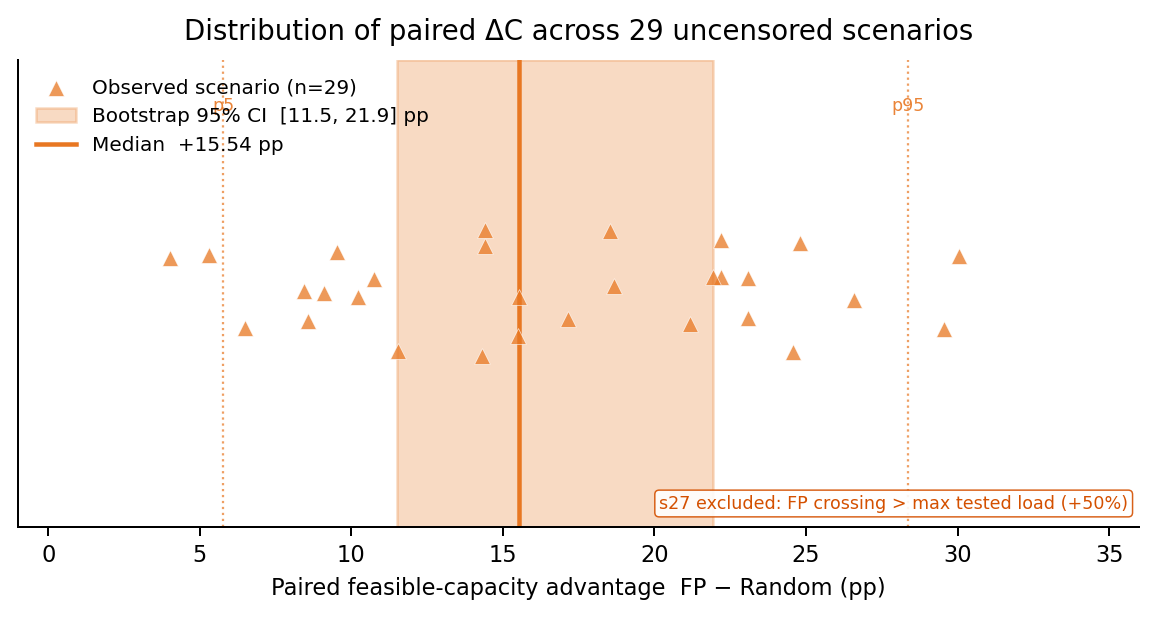
\includegraphics[width=\columnwidth]{fig_mc_dc_dist}
% Source: artifacts/phase1/figures/fig_mc_dc_dist.png (180 dpi; regenerate for camera-ready)
\caption{TODO: Capacity yield crossing illustration. The capacity headroom
percentage ($\lambda$ sweep) for fingerprint-guided and random placement,
showing the conservative bracket separation $\delta_{\mathrm{lo}}$.}
\label{fig:model}
\end{figure}

%% Section 5: Preregistered Challenge Protocol
%% STATUS: STUB — not yet drafted.
%% See artifacts/revision2/SIGMETRICS_OUTLINE.md §5 for planned content (~2 pages).

\section{Preregistered Challenge Protocol}
\label{sec:protocol}

\subsection{Preregistration}
% Scientific runner and analysis plan frozen at Git commit 5733b73.
% All comparison hypotheses, beta value, bootstrap parameters, interpretation rules
% frozen before any sc30-sc54 scenario ran.
% source: artifacts/revision2/challenge_preflight.json (plan_commit=5733b73)

\subsection{Development Context and Prespecification Timeline}
% The pre-specified challenge protocol (sc30-sc54) was designed and frozen
% after two earlier evaluation phases:
%   (1) Development runs sc0-sc4: 5 scenarios used for policy design,
%       tuning, and verification. Results not included in primary analysis.
%   (2) Earlier held-out evaluation sc5-sc29: 25 scenarios on the same base
%       dataset, using revision1 selectors (no placebos, no position template).
%       These earlier results are labeled "development-era evaluation on the
%       same underlying base dataset" (Appendix) and are not primary results.
% The frozen sc30-sc54 challenge was prespecified after sc5-sc29 was complete.
% This timeline is explicitly disclosed per the post-exposure structure in
% POST_EXPOSURE_SENSITIVITY_RECOVERY.md.

\subsection{Primary Success Criterion}
% H4 primary success: FP_vs_Random at r=1.25 achieves >= 13 of 25 held-out
% scenarios with definitely-A verdict (n_definitely_A >= 13 of 25).
% Achieved: 22/25 (n_definitely_A=22, n_indistinguishable=1, n_definitely_B=2).
% Permutation-test p-value: 1/2001 approx 0.00050 (random policy wins in
% 1 of 2001 permutations of the 25-scenario outcome).
% source: artifacts/revision2/challenge_analysis.json
%   FP_vs_Random r=1.25: n_definitely_A=22
%   interpretation.H4_primary_success.pass = true

\subsection{Preflight Gate (16/16 Conditions)}
% Before challenge execution: 16-condition preflight gate.
% source: artifacts/revision2/challenge_preflight.json
%   n_conditions=16, overall_pass=True
% Key conditions:
%   Conditions 1-12: Phase A-E completeness checks
%   Condition 14: Stage 2 full-simulation equivalence (Gate F sc0-sc4 at 1e-9 tolerance)
%   Condition 15: Analysis regression test (315/315 output cells)
%   Condition 16: Challenge seed-index audit (Amendment 5)

\subsection{LOO Cross-Fitted Beta Estimator}
% Amendment-3: per-job LOO cross-fit over 462 qualifying training jobs.
% For each job j: exclude j from fingerprint; fit per-job slope beta_{j,CF};
% PRIMARY_BETA_CHALLENGE = median_j(beta_{j,CF}) = 1.11416358 (-0.95% from frozen).
% source: artifacts/revision2/loo_beta_results.json
%   training_data.n_jobs_attempted = 462
%   B3_primary_beta.PRIMARY_BETA_CHALLENGE = 1.11416358
%   B3_primary_beta.pct_difference_from_frozen = -0.9495

% Beta estimator variants in sensitivity:
%   PRIMARY_BETA_CHALLENGE = 1.11416358 (Amendment-3 LOO cross-fit median)
%   BETA_F_FROZEN          = 1.12484352 (original frozen estimator)
%   Pooled FE slope        = 1.08293343 (superseded Amendment-2 diagnostic)
%   Legacy jackknife mean  = 1.08293397 (similar value, DIFFERENT estimator)
%   The pooled FE slope (1.08293343) and the legacy jackknife mean (1.08293397)
%   are coincidentally similar but are distinct estimators. The primary
%   estimator is the LOO CF median (1.11416358); neither 1.083 variant is primary.
%   source: artifacts/revision2/loo_beta_results.json

\subsection{Challenge Execution and Completion Audit}
% 25 scenarios (sc30-sc54); frozen commit 5733b73.
% After all scenarios: completion audit verifying completeness, seeds, hashes, NaN/Inf.
% source: artifacts/revision2/challenge_completion_audit.json (audit_pass=True, n_scenarios=25)
% Evidence freeze: commit f1c78a3.

\subsection{Post-Exposure Sensitivity Disclosure}
% E1 and E2 prespecified at 5733b73 but executed after primary results exposed.
% Design not changed after exposure.
% source: artifacts/revision2/POST_EXPOSURE_SENSITIVITY_RECOVERY.md
% source: artifacts/revision2/final_output_audit.json (post_exposure_disclosure field)

\subsection{AI-Use Disclosure}
% Per SIGMETRICS 2027 CFP requirement.
Generative-AI tools, including ChatGPT (OpenAI) and Claude/Claude Code (Anthropic),
were used for research brainstorming and methodological critique, code-generation and
debugging assistance, analysis auditing, figure-script development, and
drafting/editing. The authors made and approved all final study-design, preregistration,
analysis, and interpretation decisions; executed or supervised the analyses; verified
numerical claims against frozen artifacts; and take responsibility for all content.

%% Section 6: Primary Results
%% STATUS: STUB — table shells and figure placeholders present.
%% See artifacts/revision2/SIGMETRICS_OUTLINE.md §6 for planned content (~2.5 pages).

\section{Primary Results}
\label{sec:results}

\subsection{Primary Endpoint (H4): FP vs.\ Random at $r=1.25$}
% source: artifacts/revision2/challenge_analysis.json
%   FP_vs_Random r=1.25:
%     median_delta_lo = 6.706290619727605 -> +6.71 pp
%     bootstrap95_delta_lo = [3.9196535626004456, 8.72485557161271] -> [+3.92,+8.72]
%     n_definitely_A = 22, n_indistinguishable = 1, n_definitely_B = 2
%     interpretation.H4_primary_success.pass = true

\subsection{Node-Specificity Test: FP vs.\ Within-Cabinet Placebo}
% source: artifacts/revision2/challenge_analysis.json
%   FP_vs_WithinCabPlacebo r=1.25:
%     median_delta_lo = 3.537760317644416 -> +3.54 pp
%     bootstrap95_delta_lo = [0.5580646330144061, 4.435295391457885] -> [+0.56,+4.44]
%     n_definitely_A = 20, n_indistinguishable = 5, n_definitely_B = 0

\subsection{Factorial Comparison Table}

\begin{table}[t]
\caption{Factorial comparison results at the pre-specified $r=1.25$ choice ratio.
$\delta_{\mathrm{lo}} = C_{\mathrm{lower}}(A) - C_{\mathrm{upper}}(B)$ is the
conservative bracket separation. A: definitely A better; I: indistinguishable;
B: definitely B better. All values from 25 held-out scenarios (sc30--sc54).}
\label{tab:factorial}
\centering
\begin{tabular}{lrrr}
\toprule
Comparison & A\,/\,I\,/\,B & Median $\delta_{\mathrm{lo}}$ & Bootstrap 95\%~CI \\
\midrule
\textbf{FP vs.\ Random} (primary)        & \textbf{22\,/\,1\,/\,2}  & $+6.71$ pp & $[{+}3.92, {+}8.72]$ \\
\textbf{FP vs.\ WithinCabPlacebo}        & \textbf{20\,/\,5\,/\,0}  & $+3.54$ pp & $[{+}0.56, {+}4.44]$ \\
FP vs.\ GlobalPlacebo                    & 22\,/\,1\,/\,2            & $+4.55$ pp & $[{+}2.95, {+}7.82]$ \\
FPSpread vs.\ RandomSpread               & 20\,/\,5\,/\,0            & $+2.15$ pp & $[{+}0.52, {+}4.25]$ \\
RandomSpread vs.\ Random                 & 8\,/\,14\,/\,3            & $+0.00$ pp & $[{-}0.26, {+}0.03]$ \\
FPSpread vs.\ FP                         & 4\,/\,3\,/\,18            & $-2.64$ pp & $[{-}4.49, {-}2.00]$ \\
FP vs.\ PositionTemplate                 & 16\,/\,5\,/\,4            & $+0.74$ pp & $[{-}0.82, {+}1.50]$ \\
FPSpread vs.\ PositionTemplate           & 6\,/\,11\,/\,8            & $-1.16$ pp & $[{-}2.29, {-}0.25]$ \\
\bottomrule
\end{tabular}
% source: artifacts/revision2/challenge_analysis.json (all rows verified in
%         FINAL_NUMERICAL_CLAIM_AUDIT.md V8-V24)
% Floor/left-censored note for FP_vs_Random:
%   full_random: 9 base-infeasible (left_boundary, [0,0]) + 3 floor-at-zero (exact_bracket, C_lower=0) = 12 total C_lower=0
%   full_fp: 0 base-infeasible, 0 floor
%   n_both_left_censored: 0 (FP never base-infeasible at r=1.25)
%   First binding constraint for random base-infeasible scenarios: B=8, S=1
% RandomSpread_vs_Random n_both_left_censored: 6 (both policies base-infeasible in same 6 scenarios)
% These scenarios are not "ties at zero"; they are base-infeasible and excluded from bracket-width summaries.
% source: per-scenario crossing data in artifacts/revision2/results/gate_f_sc*_all_r2challenge.json
\end{table}

\subsection{Factorial Pattern Interpretation}
% TODO: Discuss interpretation — global placebo, spreading decomposition,
% negative control, position template non-separation.

% Figure 3: Primary challenge forest plot
\begin{figure}[t]
\centering
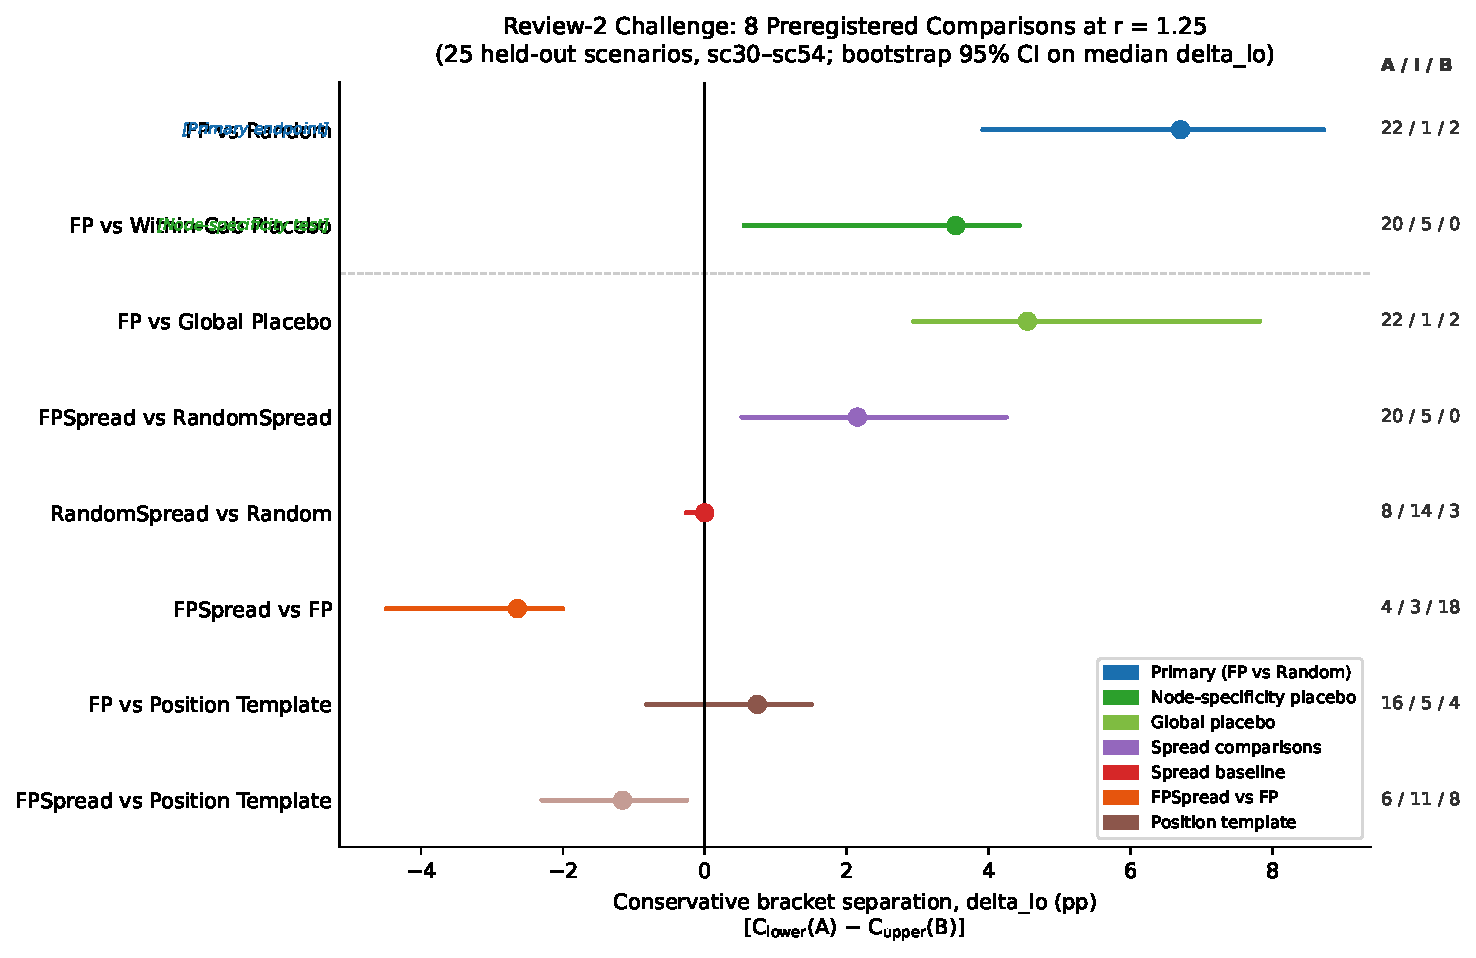
\includegraphics[width=0.85\textwidth]{fig_r2_factorial_r125}
% source: artifacts/revision2/figures/fig_r2_factorial_r125.pdf (300 dpi)
% generation: artifacts/revision2/figures/fig_r2_main.py
\caption{Forest plot of 8 pre-specified comparisons at $r=1.25$.
Each row shows the median conservative bracket separation $\delta_{\mathrm{lo}}$
with bootstrap 95\%~CI. A/I/B counts (definitely-A / indistinguishable /
definitely-B) shown at right. All 25 held-out scenarios (sc30--sc54).}
\label{fig:factorial}
\end{figure}

\subsection{Pre-specified Secondary Finding: FPSpread Crossover}

% Figure 4: FPSpread crossover
\begin{figure}[t]
\centering
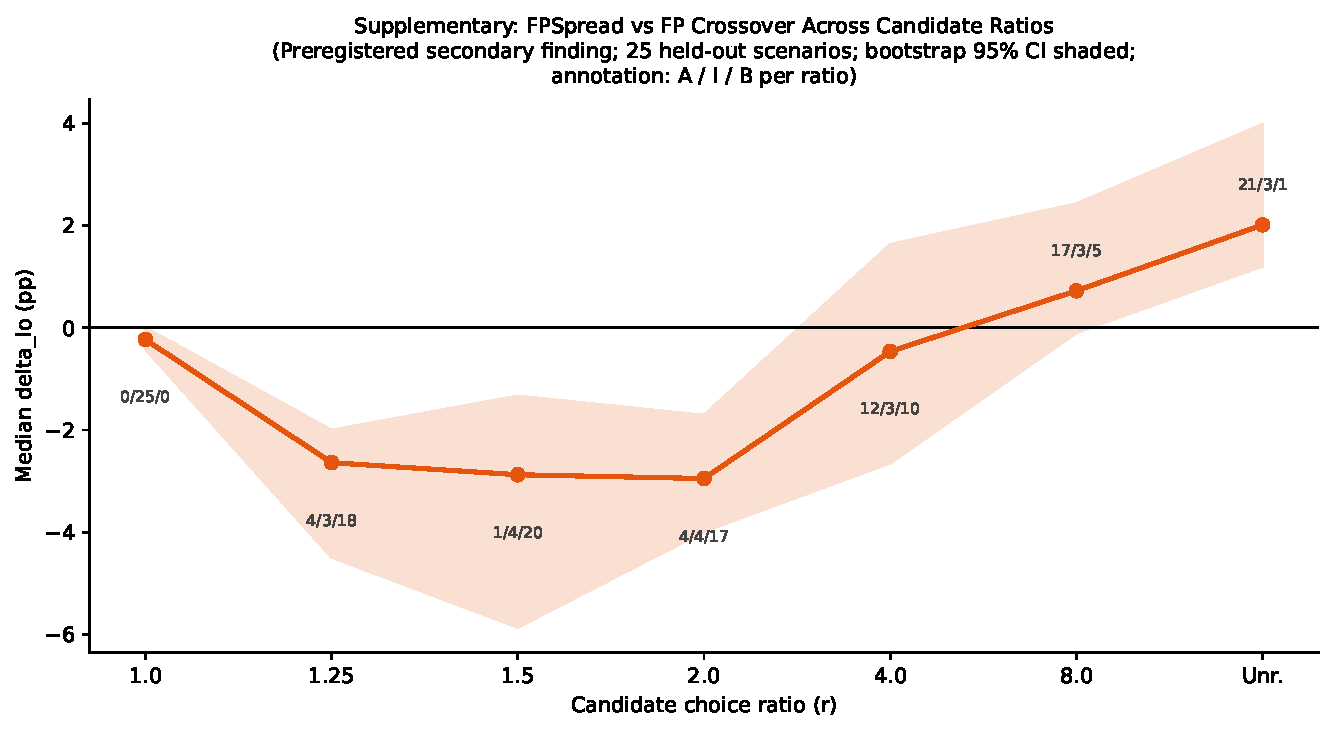
\includegraphics[width=0.75\textwidth]{fig_r2_fpspread_crossover}
% source: artifacts/revision2/figures/fig_r2_fpspread_crossover.pdf (300 dpi)
% generation: artifacts/revision2/figures/fig_r2_main.py
\caption{FPSpread vs.\ FP across candidate choice ratios (pre-specified secondary finding). FPSpread underperforms FP at constrained ratios ($r=1.25$--$2.0$) and
outperforms at large choice sets ($r\geq8.0$, unrestricted). Values from
challenge\_analysis.json; shaded region is bootstrap 95\%~CI.}
\label{fig:crossover}
\end{figure}

% source for crossover table: artifacts/revision2/challenge_analysis.json
%   FPSpread_vs_FP r=1.25: -2.640 pp  (4/3/18)
%   FPSpread_vs_FP r=1.5:  -2.876 pp  (1/4/20)
%   FPSpread_vs_FP r=2.0:  -2.951 pp  (4/4/17)
%   FPSpread_vs_FP r=4.0:  -0.464 pp  (12/3/10)
%   FPSpread_vs_FP r=8.0:  +0.722 pp  (17/3/5)
%   FPSpread_vs_FP unr:    +2.012 pp  (21/3/1)

\subsection{Negative Control}
% All 8 comparisons at r=1.0: 0 / 25 / 0.
% source: artifacts/revision2/challenge_analysis.json
%   H5_r1_negative_control.all_indistinguishable = true

%% Section 7: Robustness and Sensitivity Analysis
%% STATUS: STUB — figure placeholder and table shell present.
%% See artifacts/revision2/SIGMETRICS_OUTLINE.md §7 for planned content (~2 pages).

\section{Robustness and Sensitivity Analysis}
\label{sec:robustness}

\subsection{E1: Cabinet-Envelope Scale Sensitivity}
% source: artifacts/revision2/sensitivity_cabinet_scale.json
%   5 scale factors [0.90, 0.95, 1.00, 1.05, 1.10], FP_vs_Random at r=1.25
%   0.90: +0.814 pp [+0.002, +2.381]  18/6/1
%   0.95: +2.977 pp [+0.547, +4.278]  21/4/0
%   1.00: +6.706 pp [+3.920, +8.725]  22/1/2 (primary)
%   1.05: +4.404 pp [+3.202, +5.536]  20/3/2
%   1.10: +4.687 pp [+0.871, +5.330]  20/2/3
%   Result: sign positive at all 5 scale factors
% Note: at scale=0.90, CI barely clears zero ([+0.002, +2.381]).
% Post-exposure disclosure applies (see §5).

\subsection{E2: Beta Sensitivity}
% source: artifacts/revision2/sensitivity_loo_beta.json
%   6 beta values: primary (1.114), frozen (1.125), prospective (0.96),
%                  jackknife (1.083), CF-P5 (1.066), CF-P95 (1.169)
%   All medians positive; no sign reversal. Result: stable (no sign reversal).
% Post-exposure disclosure applies (see §5).

\begin{table}[t]
\caption{E1/E2 sensitivity analysis results. Panel A (E1): FP vs.\ Random at
$r=1.25$ across five cabinet-envelope scale factors; sign positive at all five. Panel B (E2):
across six pre-specified beta estimator variants; no sign reversal. Post-exposure
disclosure: E1/E2 were prespecified at commit 5733b73 but executed after primary
results were exposed; design was not changed.}
\label{tab:sensitivity}
\centering
\begin{tabular}{lrrr}
\toprule
& n\,/\,I\,/\,B & Median $\delta_{\mathrm{lo}}$ & Bootstrap 95\%~CI \\
\midrule
\multicolumn{4}{l}{\textit{Panel A --- E1: Cabinet scale}} \\
Scale 0.90 & 18\,/\,6\,/\,1 & $+0.81$ pp & $[{+}0.002, {+}2.38]$ \\
Scale 0.95 & 21\,/\,4\,/\,0 & $+2.98$ pp & $[{+}0.55, {+}4.28]$ \\
\textbf{Scale 1.00 (primary)} & \textbf{22\,/\,1\,/\,2} & $+6.71$ pp & $[{+}3.92, {+}8.72]$ \\
Scale 1.05 & 20\,/\,3\,/\,2 & $+4.40$ pp & $[{+}3.20, {+}5.54]$ \\
Scale 1.10 & 20\,/\,2\,/\,3 & $+4.69$ pp & $[{+}0.87, {+}5.33]$ \\
\midrule
\multicolumn{4}{l}{\textit{Panel B --- E2: Beta value}} \\
\textbf{Primary (LOO CF, 1.114)} & \textbf{22\,/\,1\,/\,2} & $+6.71$ pp & $[{+}3.92, {+}8.72]$ \\
Frozen (1.125)        & 22\,/\,1\,/\,2 & $+6.48$ pp & $[{+}3.92, {+}8.72]$ \\
2025 in-sample (0.960) & 22\,/\,1\,/\,2 & $+6.67$ pp & $[{+}2.08, {+}7.04]$ \\
Jackknife (1.083)     & 22\,/\,1\,/\,2 & $+5.59$ pp & $[{+}3.92, {+}8.72]$ \\
CF P5 (1.066)         & 21\,/\,2\,/\,2 & $+6.42$ pp & $[{+}3.20, {+}8.72]$ \\
CF P95 (1.169)        & 22\,/\,1\,/\,2 & $+5.35$ pp & $[{+}2.16, {+}8.72]$ \\
\bottomrule
\end{tabular}
% source Panel A: artifacts/revision2/sensitivity_cabinet_scale.json
% source Panel B: artifacts/revision2/sensitivity_loo_beta.json
\end{table}

% Figure 5: Robustness panels (E1 + E2)
\begin{figure}[t]
\centering
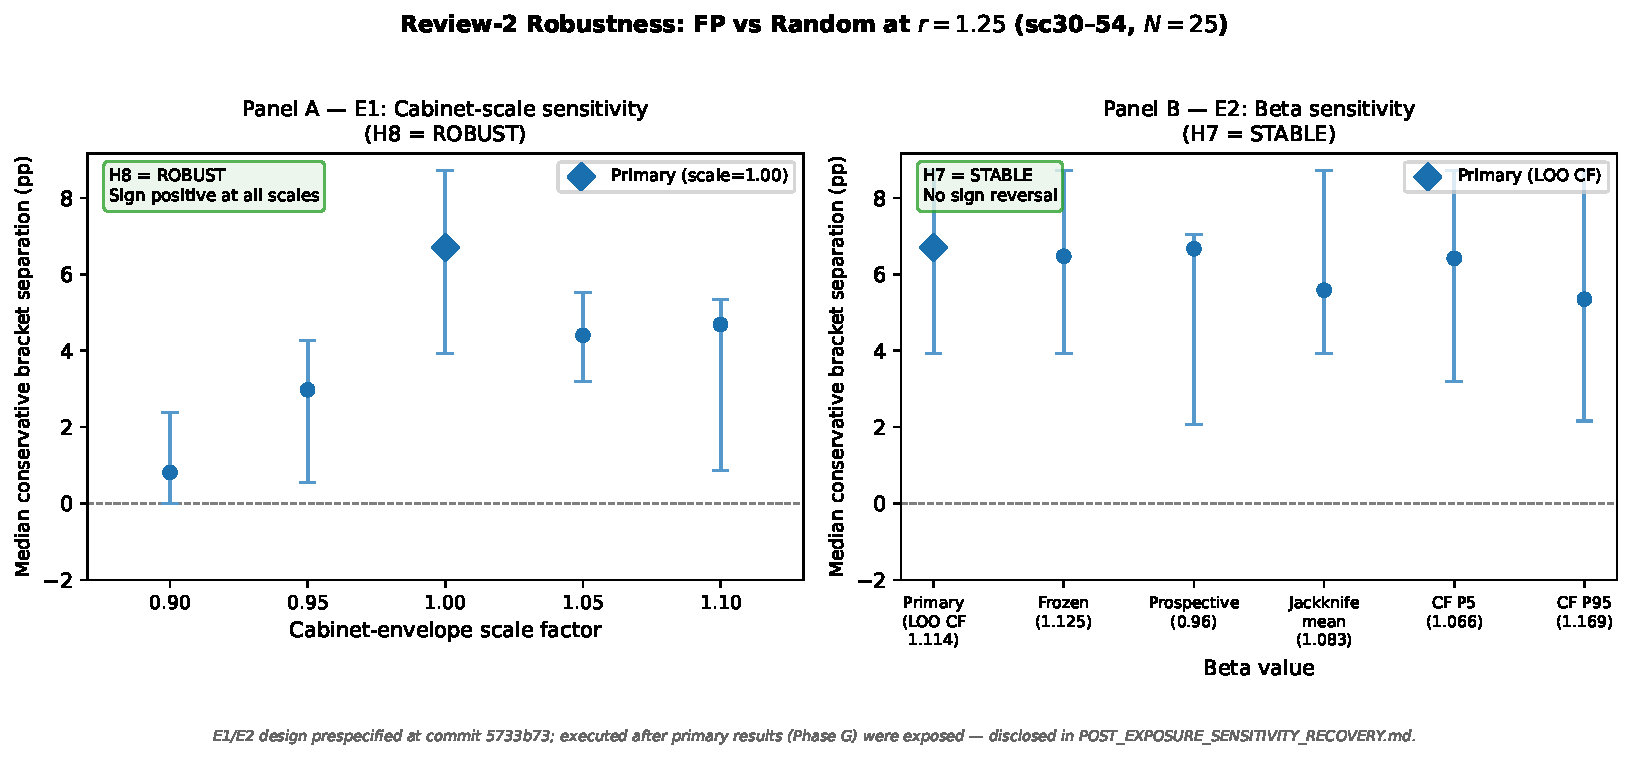
\includegraphics[width=\textwidth]{fig_r2_robustness}
% source: artifacts/revision2/figures/fig_r2_robustness.pdf (300 dpi)
% generation: artifacts/revision2/figures/fig_r2_robustness.py
\caption{Robustness analysis. Panel A (E1): FP vs.\ Random median
$\delta_{\mathrm{lo}}$ (pp) across five cabinet-envelope scale factors
$[0.90, 1.10]$; sign positive at all scales; barely clearing
zero at $-10\%$). Panel B (E2): across six pre-specified beta estimator
variants; no sign reversal. Primary value highlighted (diamond).
Error bars: bootstrap 95\%~CI.}
\label{fig:robustness}
\end{figure}

%% Section 8: Discussion and Limitations
%% STATUS: STUB — key limitation topics outlined.
%% See artifacts/revision2/SIGMETRICS_OUTLINE.md §8 for planned content (~1.5 pages).

\section{Discussion and Limitations}
\label{sec:discussion}

\subsection{Scope: Constraint-Aware Replay Model}
% All results are within the replay model. The +6.71 pp advantage is a capacity-yield
% separation in the replay model — not observed live throughput improvement.
% Node-hours translation: algebraic (78,907 base cohort node-hours × [0.036, 0.056])
% -> ~2,800-4,400 additional cohort node-hours per replay window.
% This is a replay-model algebraic translation, not observed output.
% source: artifacts/phase1/analysis/phase3b_mc_results.json (H_cohort_hist_nh=78907.3775)

\subsection{T\_thr Not Directly Tested}
% Thermal threshold T_thr = 63.625C (primary) / 60.602C (secondary) was fixed
% at Gate F calibration and not varied in Review-2.
% E1 (cabinet-scale sensitivity) tests a different calibration dimension.
% T_thr sensitivity is a documented limitation.

\subsection{Monte Carlo vs.\ Data Uncertainty}
% The capacity-yield separation is measured through replay-model simulation,
% not from empirical before/after operational data. The bootstrap quantifies
% uncertainty in the scenario-to-scenario ranking (25 random draws from a
% fixed base workload with fixed fingerprints). It does not quantify:
%   (1) uncertainty in the fingerprint estimates themselves (FA_2024 is
%       computed from a finite training set; out-of-distribution workloads
%       may not induce the same thermal ordering);
%   (2) uncertainty from replay vs. live execution (live scheduling interacts
%       with job start times, preemption, and node failures not captured in replay);
%   (3) model-definition sensitivity (cabinet-reference definition; threshold T_thr).
% The +6.71 pp advantage is a replay-model measurement with quantified
% scenario-level uncertainty; it is not a Monte Carlo estimate of a population
% parameter, and it is not confirmed by paired live A/B operational data.

\subsection{Network Locality and Runtime Effects}
% Frontier jobs are assigned in contiguous rack groups for network locality.
% The fingerprint selector operates within a candidate set of size r=1.25×k,
% where k is the requested node count. At constrained ratios (r=1.25),
% the thermal-aware selector may conflict with topological locality preferences:
% the coolest available nodes may not form a contiguous network-local allocation.
% Potential effects: (1) communication overhead from non-contiguous placement
% (not measured); (2) interference between thermal-aware and topology-aware
% objectives in a production multi-policy scheduler. The replay model does not
% model network locality beyond cabinet-level span (cab_span_median = 9 cabinets
% for FP at r=1.25; see policy_summaries in challenge_analysis.json).
% r=1.25 is not interpreted as modeling a specific locality regime; it is the
% pre-specified primary ratio from the frozen challenge protocol.

\subsection{Position Template Non-Separation}
% FP not statistically separated from thermally informed structural-position template
% at the primary choice ratio (16/5/4, median +0.74 pp, CI [-0.82, +1.50]).
% source: artifacts/revision2/challenge_analysis.json
% The position template reflects average historical fingerprint at each physical position.
% We do not claim fingerprints outperform all thermally informed strategies.

\subsection{Fleet Generalizability}
% Study cohort: 2,000 nodes (20.3% of Frontier's 9,856 nodes).
% Result applies to the study cohort under the historical operating envelope.
% Extrapolation to full-fleet deployment is not validated.
% Three late-arriving cabinets (2600-2602): documented calibration concern.
% source: artifacts/revision2/cabinet_timeline_audit.json

\subsection{Post-Exposure Sensitivity Disclosure}
% E1/E2 prespecified at commit 5733b73 but executed after Phase G primary results
% exposed. Design not changed after exposure.
% source: artifacts/revision2/POST_EXPOSURE_SENSITIVITY_RECOVERY.md

\subsection{AI-Use Disclosure}
% See §\ref{sec:protocol} for full AI-use disclosure per SIGMETRICS 2027 CFP.

%% Section 9: Conclusion
%% STATUS: STUB — not yet drafted.
%% See artifacts/revision2/SIGMETRICS_OUTLINE.md §9 for planned content (~0.5 pages).

\section{Conclusion}
\label{sec:conclusion}

% TODO: Draft conclusion summarizing:
% 1. Thermal fingerprints are a durable, measurable property of individual nodes
%    (r=0.926, R2=0.848 prospective; calendar-year timescale).
% 2. Fingerprint-aware placement provides held-out scheduling-capacity advantage
%    beyond cabinet-level composition (+6.71 pp vs random; +3.54 pp vs within-cab placebo).
% 3. Results are robust to ±10% calibration error and stable across 6 beta variants.
% 4. The FPSpread crossover is a preregistered secondary finding with implications
%    for choice-set-size-aware scheduling policy design.
% 5. Open questions: T_thr sensitivity; position template mechanism; causal physical
%    mechanism for fingerprint persistence; full-fleet deployment.


%% ---- Bibliography -------------------------------------------------------
\bibliographystyle{ACM-Reference-Format}
\bibliography{references}

\end{document}
